\documentclass[a4paper,11pt]{article}
\usepackage[utf8]{inputenc}
\usepackage{graphicx}
\usepackage{enumerate}
\usepackage{geometry}
\usepackage{fancyhdr}
\usepackage{minted}
\usepackage{xcolor}
\usepackage{listings}
\usepackage[colorlinks = true,
            linkcolor = blue,
            urlcolor  = blue,
            citecolor = blue]{hyperref}

\geometry{total={210mm,297mm},
left=25mm,right=25mm,%
bindingoffset=0mm, top=20mm,bottom=20mm}

\graphicspath{ {./images/} }
\renewcommand{\thesubsection}{\thesection.\alph{subsection}}
\renewcommand*\sfdefault{phv}
\renewcommand\familydefault{\sfdefault}

% \renewcommand{\thesubsubsection}{\thesubsection.\alph{subsubsection}}

% \newmintedfile{html}{
%     linenos,
%     breaklines,
%     python3,
%     numbersep=8pt,
%     frame=single,
%     framesep=3mm} 

\newcommand*{\TitleFont}{%
      \usefont{\encodingdefault}{\rmdefault}{b}{n}%
      \fontsize{16}{20}%
      \selectfont}

\linespread{1.3}

% my own titles
\makeatletter
\renewcommand{\maketitle}{
\begin{center}
\vspace{2ex}
{\huge \textsc{\@title}}
\vspace{1ex}
\\
\rule{\linewidth}{0.5pt}\\
\@author \hfill \@date
\vspace{4ex}
\end{center}
}
\makeatother

\definecolor{bg}{rgb}{0.95,0.95,0.95}


% custom footers and headers
\pagestyle{fancy}
\lhead{}
\chead{}
\rhead{}
\lfoot{Assignment 6 : Computer Architecture }
\cfoot{}
\rfoot{Page \thepage}
\renewcommand{\headrulewidth}{0pt}
\renewcommand{\footrulewidth}{0pt}
%%----------%%%----------%%%----------%%%----------%%%

\begin{document}

\newminted{ssembly}{fontsize=\scriptsize, 
    linenos,
    numbersep=8pt,
    frame=single,
    bgcolor=bg,
    framesep=3mm} 

\newminted{bash}{fontsize=\scriptsize, 
    linenos,
    python3,
    numbersep=8pt,
    frame=single,
    bgcolor=bg,
    framesep=3mm}


% \newminted{all}{linenos, frame=single}

% \usemintedstyle{monokai}
\usemintedstyle{manni}
% \usemintedstyle{xcode}
% \usemintedstyle{vs}
% \usemintedstyle{autumn}
% \usemintedstyle{colorful}
% \usemintedstyle{trac}


\title{ \TitleFont Assignment 6 : Computer Architecture }

\author{Emil Sharifulllin, Innopolis University}

\date{\today}

\maketitle
\tableofcontents

\section{Digital Circuit}

\subsection{Draw a digital circuit of an 4-bit incrementer, i.e., a circuit that satisfies the equation b = a + 1 mod 24. You can use the operations from the set \{and, or, nand, nor, not, xor\}.}

I decided, that incrementor is looks like an adder but second number contains only one bit. Also carry from every half-incrementor should be connected with following half-incrementor like an one of inputs. My incrementor have following circuit:

\begin{center}
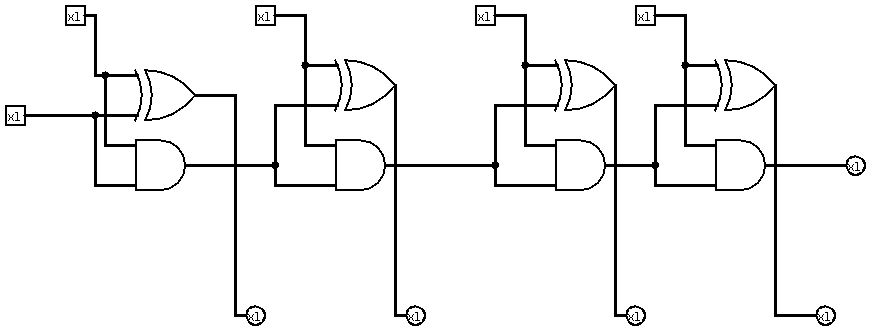
\includegraphics[width=15cm]{incrementor}
\end{center}

\subsection{Try to find an incrementer with the minimal number of operations needed.}
As we have always 1 as second number, so we can delete first AND. Also we can delete last AND instruction if it's not matter to measure carry after increment. So minimal incrementor contain 6 elements.

\section{Experiments Performance measurement}
\subsection{}
I downloaded simulator and measured programs given in gomponents.

\subsection{}
\subsubsection{The number of instructions that have been executed for every architecture.}
\begin{center}
\begin{tabular}{|c|c|c|c|}
\hline
Program/Architecture & MultiCycle & SingleCycle & Pipelined  \\ \hline \hline 
addition & 6 & 6 & 100  \\ \hline 
forloop & 45 & 46 & 135  \\ \hline 
squares & 101 & 101 & 131  \\ \hline 
\end{tabular}
\end{center}

\subsubsection{The CPI}
\begin{center}
\begin{tabular}{|c|c|c|c|}
\hline
Program/Architecture & MultiCycle & SingleCycle & Pipelined  \\ \hline \hline 
addition & 3.7 & 1 & 1  \\ \hline 
forloop & 3.6 & 1 & 1  \\ \hline 
squares & 3.6 & 1 & 1  \\ \hline 
\end{tabular}
\end{center}

\subsubsection{The CPU time}
If we assume that we have 1Hz processor, this programs will execute following times:
\begin{center}
\begin{tabular}{|c|c|c|c|}
\hline
Program/Architecture & MultiCycle & SingleCycle & Pipelined  \\ \hline \hline 
addition & 0.002 & 0.003 & 0.01  \\ \hline 
forloop & 0.016 & 0.023 &  0.014 \\ \hline 
squares & 0.035 & 0.051 &  0.013 \\ \hline 
\end{tabular}
\end{center}

\subsection{Explain the following:}
\subsubsection{Which architecture performed the best for every executable and explain why}
\begin{itemize}
  \item \textbf{addition - } MultiCycle is the best because a lot of instructions contains a few operations.
  \item \textbf{forloop - } Pipelined is the pest because this architecture can start to operate with next instruction whule previous currently operates.
  \item \textbf{squares - } SingleCycle is the best because this program contains a lot of smal instructions.
\end{itemize}
\subsubsection{A program counter is present in the architecture. Can you explain what the program counter function is?}
The function of PC is to point to current or next instruction.
\subsubsection{What do you notice about the behavior when running a simulation?}
I predicted same behaviour as I saw in simulation. SingleCycle and pipelined architectures have CPI = 1 and MyltiCycle have overage CPI 3.5.

\subsection{In the programs there are different instructions. Explain for the following instructions what  do they do and how the are used.}
\subsubsection{ADDI}
\textbf{Add immediate} Adds a register and a sign-extended immediate value and stores the result in a register. 
\subsubsection{NOP}
\textbf{No operation} Tells to processor to do nothing
\subsubsection{LI}
\textbf{Load immediate} Emulator instruction that writes lower two bytes of number to register.
\subsubsection{BNE}
\textbf{Branch on not equal} Branches if the two registers are not equal
\subsection{Now change the first program to subtract two numbers, do not change the initialization of the  variables can you explain what happens.}

\begin{bashcode}
LI  $4, 1
ADD   $1, $4, $0
LI  $5, 2
ADD   $2, $5, $0
SUB   $6, $1, $2
ADD   $3, $6, $0
\end{bashcode}

After execution of this program register 3 will have value 0xFFFFFFFF because 1-2 is equal to -1.

\subsection{Finally explain why the clock rate (frequency) of a cpu is not a good benchmark for the  performance of a cpu.}
Sometimes for example CPU's with pipeline architecture requires instructuions that not depends on previous instructions and if 

\end{document}